
\chapter{\textgreek{Εισαγωγή}}
\label{chapter_1}
%\pagestyle{empty}
\pagestyle{fancy}
\fancyhf{}
%\fancyhead[OC]{\leftmark}
%\fancyhead[C]{}
%\fancyhead[EC]{\rightmark}
\renewcommand{\footrulewidth}{0.5pt}
\cfoot{\thepage}

%\begin{flushleft}

\section{\textgreek{Μηχανική Μάθηση και Σημασιολογική Κατάτμηση}}
\textgreek{Μηχανική Μάθηση είναι ένας τομέας ο οποίος ανήκει στην Επιστήμη των Υπολογιστών ο οποίος επικεντρώνεται σε εκλεπτυσμένους αλγορίθμους οι οποίοι δεν έχουν δημιουργηθεί ρητά από τους επιστήμονες, αλλά μαθαίνουν από τα δεδομένα και προσαρμόζονται σε αυτά για να κάνουν προβλέψεις ή για να πάρουν αποφάσεις. Τα τελευταία χρόνια η εξέλιξη της υπολογιστικής δύναμης καθώς και ο μεγάλος όγκος δεδομένων που είναι διαθέσιμος επιτρέπει στους επιστήμονες να πειραματιστούν με πιο πολύπλοκους αλγόριθμους. Ο συγκεκριμένος κλάδος καλύπτει ένα μεγάλο εύρος εφαρμογών, από μηχανές αναζήτησης} [\citenum{7538344}]\textgreek{ και μετάφραση κειμένου }\cite{machine_translation}\textgreek{ μέχρι εκτιμήσεις για ασθένειες στον κλάδο της Ιατρικής} \cite{medical_pred}.

% Σε αυτή την εργασία, αποφασίσαμε να επικεντρωθούμε στο θέμα της Σημασιολογικής Κατάτμησης από εικόνες αστικών περιοχών.
%\subsubsection{Data and Description}
%\lhead{}
\section{\textgreek{Σημασιολογική Κατάτμηση και Αναγνώριση Αντικειμένων}}
\textgreek{Στην Επιστήμη των Υπολογιστών υπάρχει μια διαφοροποιήση μεταξύ ενός προβλήματος αναγνώρισης αντικειμένων και ενός προβλήματος Σημασιολογικής Κατάτμησης αντικειμένων. Αυτά τα δύο προβλήματα ενώ στην ουσία αποσκοπούν στον ίδιο στόχο, έχουν μια πολύ σημαντική διαφορά. Όταν μιλάμε για αναγνώριση αντικειμένων δεν αναφερόμαστε στην ακριβή εύρεση της τοποθεσίας ενός αντικειμένου στην εικόνα αλλά στη γενική του μορφή, δηλαδή χωρίς την ακριβή εύρεση των ορίων του αντικειμένου (εικόνα} \ref{fig:yolo_img}). \textgreek{Εν αντιθέσει, στο θέμα της Σημασιολογικής Κατάτμησης αντικειμένων, μας ενδιαφέρει η τοποθεσία ενός αντικειμένου στην εικόνα αλλά και η εύρεση των ακριβών ορίων του αντικειμένου, καθώς τοποθετούμε κάθε εικονοστοιχείο της εικόνας σε μια κατηγορία αντικειμένου (εικόνα} \ref{fig:seg_img}). \\[2cm] \textgreek{Στις παρακάτω εικόνες φαίνονται ξεκάθαρα οι διαφορές των 2 προβλημάτων.}

\begin{figure}[h!]
\centering
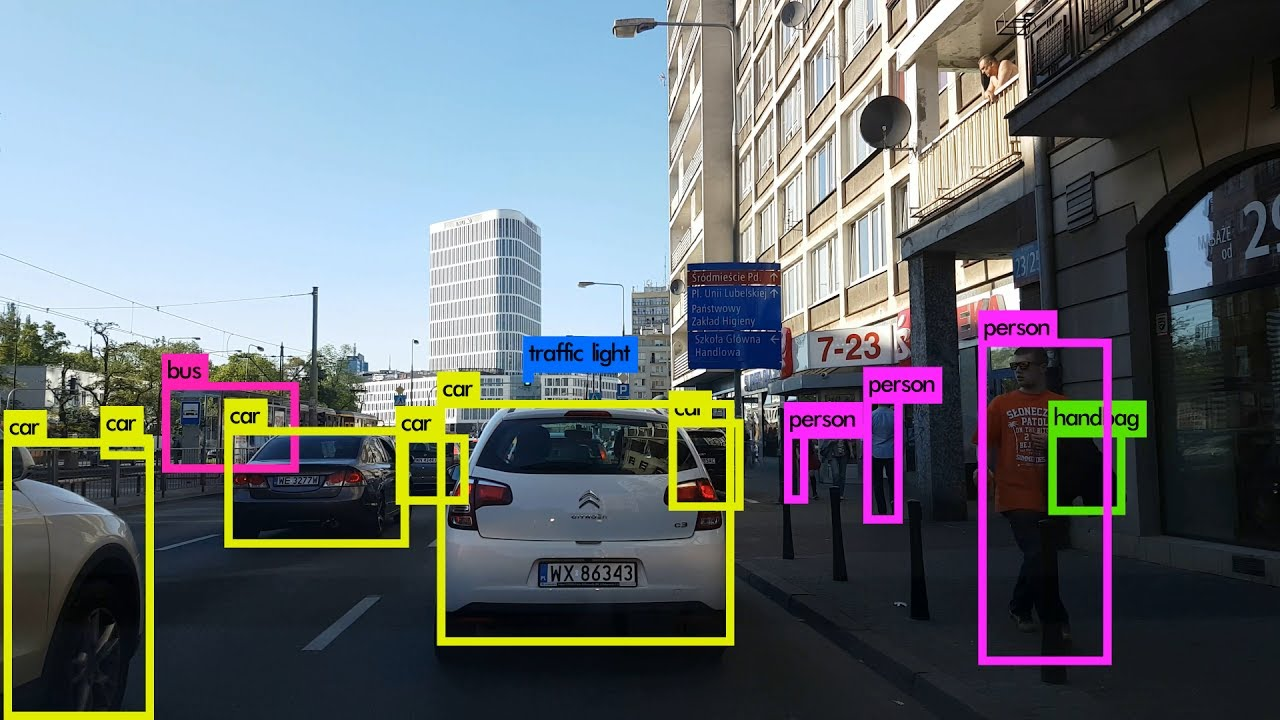
\includegraphics[scale=0.3]{Images/Obj_det}
\caption[\textgreek{Αναγνώριση} YOLO]{\textgreek{Παράδειγμα ενός συστήματος αναγνώρισης αντικειμένων. Αποτέλεσμα του συστήματος }YOLO \cite{yolo}}
\label{fig:yolo_img}
\end{figure}

\begin{figure}[h!]
\centering
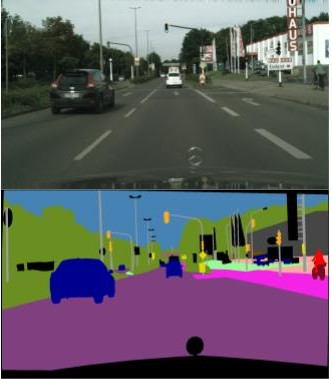
\includegraphics{Images/seg}
\caption[\textgreek{Παράδειγμα Σημασιολογίας}]{\textgreek{Παράδειγμα ενός συστήματος Σημασιολογικής Κατάτμησης αντικειμένων από εικόνες.}}
\label{fig:seg_img}
\end{figure}

\section{\textgreek{Η Βάση Δεδομένων} Cityscapes }
\textgreek{Σε αυτή την εργασία χρησιμοποιήθηκε η βάση δεδομένων} \href{https://www.cityscapes-dataset.com/} {Cityscapes} \cite{Cityscapes} \textgreek{η οποία αποτελείται από ένα σύνολο έγχρωμων εικόνων υψηλής ευκρίνειας τραβηγμένες σε αστικές περιοχές. Περιλαμβάνει 19 κατηγορίες αντικειμένων ενώ διαθέτει και μία επιπλέον κατηγορία για την ταξινόμηση των αντικειμένων που δεν ανήκουν σε καμία κατηγορία. Τα αντικείμενα στις εικόνες έχουν επισημειωθεί σε επίπεδο εικονοστοιχείου. Δηλαδή, όλα τα εικονοστοιχεία της εικόνας ανήκουν σε κάποιο αντικείμενο. Η βάση περιέχει περισσότερες από 5000 εικόνες μεγέθους 1024}x\textgreek{2048 εικονοστοιχείων από 50 πόλεις της Ευρώπης. Οι εικόνες έχουν τραβηχτεί από μια κάμερα ακολουθιακά με διάστημα ενός δευτερολέπτου μεταξύ τους.}
\\[1cm]
\textgreek{Το σύνολο δεδομένων διαθέτει επίσης ένα άλλο κομμάτι το οποίο αποτελείται από 20000 εικόνες των οποίων τα εικονοστοιχεία έχουν επισημειωθεί πιο αφηρημένα. Οι παρακάτω εικόνες δείχνουν τη διαφορά μεταξύ των δύο συνόλων, οι μερικώς επισημειωμένες εικόνες δεν έχουν όλα τα εικονοστοιχεία ταξινομημένα. Το συγκεκριμένο σύνολο από εικόνες δεν έχει χρησιμοποιηθεί στα πειράματά μας.}

\begin{figure}[h!]
 \centering
 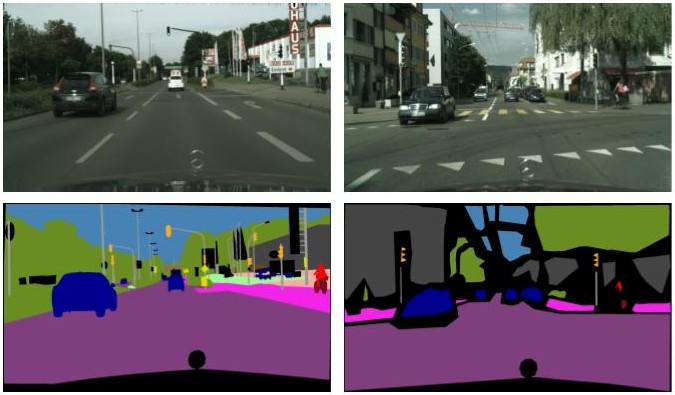
\includegraphics[scale=0.6]{Images/dataset.jpg}
 \caption[\textgreek{Παράδειγμα Εικόνων Βάσης}]{\textgreek{Αριστερά: Πλήρως επισημειωμένες εικόνες.
 \\ Εικόνα Δεξιά: Μερικώς επισημειωμένες εικόνες.}}
\end{figure}


%\{Semantics Segmentation Applications}

\subsection{\textgreek{Περιγραφή Αντικειμένων}}
\textgreek{Η βάση περιέχει 19 αντικείμενα τα οποία ανήκουν σε 6 υπερ-κατηγορίες. Τα εικονοστοιχεία που ανήκουν σε κατηγορίες αντικειμένων που δεν μας αφορούν στην διαδικασία της αναγνώρισης είναι σημειωμένα ως} \emph{\textgreek{`Χωρίς Ετικέτα`}}. \textgreek{Αυτά τα αντικείμενα πιο αναλυτικά είναι:}
\\[1cm]
\[
\begin{array}{lccc}
 \text{Classes} &\text{\textgreek{Κλάσεις}} & \text{Categories} &\text{\textgreek{Κατηγορίες}}\\
 \hline
 
 \text{Road} 		&\text{\textgreek{Δρόμος}} & 	\text{Flat} &\text{\textgreek{Επίπεδο}}\\
 \text{Sidewalk} 	&\text{\textgreek{Πεζοδρόμιο}} & \text{Flat} &\text{\textgreek{Επίπεδο}}\\
 \text{Building} 	&\text{\textgreek{Κτίριο}} & 	\text{Construction} &\text{\textgreek{Κατασκευή}}\\
 \text{Wall} 		&\text{\textgreek{Τοίχος}} & 	\text{Construction} &\text{\textgreek{Κατασκευή}}\\
 \text{Fence} 		&\text{\textgreek{Φράχτης}} & 	\text{Construction} &\text{\textgreek{Κατασκευή}}\\
 \text{Pole} 		&\text{\textgreek{Ιστός}} & 	\text{Object} &\text{\textgreek{Αντικείμενο}}\\
 \text{Traffic light} 	&\text{\textgreek{Φανάρι κυκλοφορίας}} & \text{Object} &\text{\textgreek{Αντικείμενο}}\\
 \text{Traffic sign} 	&\text{\textgreek{Πινακίδα κυκλοφορίας}} & \text{Object} &\text{\textgreek{Αντικείμενο}}\\
 \text{Vegetation} 	&\text{\textgreek{Βλάστηση}} & 		\text{Nature} &\text{\textgreek{Φύση}}\\
 \text{Terrain} 	&\text{\textgreek{Έδαφος}} & 		\text{Nature} &\text{\textgreek{Κατηγορίες}}\\
 \text{Sky} 		&\text{\textgreek{Ουρανός}} & 		\text{Sky} &\text{\textgreek{Ουρανός}}\\
 \text{Person} 		&\text{\textgreek{Άνθρωπος}} &		\text{Human} &\text{\textgreek{Άνθρωπος}}\\
 \text{Rider} 		&\text{\textgreek{Αναβάτης}} & 		\text{Human} &\text{\textgreek{Άνθρωπος}}\\
 \text{Car} 		&\text{\textgreek{Αυτοκίνητο}} & 	\text{Vehicle} &\text{\textgreek{Όχημα}}\\
 \text{Truck} 		&\text{\textgreek{Φορτηγό}} & 		\text{Vehicle} &\text{\textgreek{Όχημα}}\\
 \text{Bus} 		&\text{\textgreek{Λεωφορείο}} & 	\text{Vehicle} &\text{\textgreek{Όχημα}}\\
 \text{Train} 		&\text{\textgreek{Τρένο}} & 		\text{Vehicle} &\text{\textgreek{Όχημα}}\\
 \text{Motorcycle} 	&\text{\textgreek{Μοτοσυκλέτα}} & 	\text{Vehicle} &\text{\textgreek{Όχημα}}\\
 \text{Bicycle} 	&\text{\textgreek{Ποδήλατο}} & 		\text{Vehicle} &\text{\textgreek{Όχημα}}\\
 \text{Unlabeld} 	&\text{\textgreek{Χωρίς Ετικέτα}} & 	\text{Void} &\text{\textgreek{Κενό}}\\
  \hline
\end{array}
\]
%

\section{\textgreek{Με μια Ματιά}}
\subsection{\textgreek{Στόχοι Διπλωματικής}}
\textgreek{Ο σκοπός αυτής της Διπλωματικής είναι να μελετήσουμε το πρόβλημα της Σημασιολογικής Κατάτμησης Έγχρωμων Εικόνων οι οποίες αναπαριστούν αστικά περιβάλλοντα με την χρήση μεθόδων μηχανικής μάθησης. Η προσπάθειά μας στοχεύει στην πλήρη και ολοκληρωμένη ανασκόπηση ορισμένων από τους αλγορίθμους και τα εργαλεία που θα μπορούσαν να χρησιμοποιηθούν σε αυτόν τον συγκεκριμένο τομέα καθώς και στη σύγκριση των διαφόρων μεθόδων ταξινόμησης. Η δουλειά μας βασίζεται στην έρευνα που δημοσιεύτηκε στον ιστότοπο του }Cityscapes-Dataset \textgreek{προκειμένου να αποκτηθούν γνώσεις στον τομέα και ως εκ τούτου να επεκτείνουμε αυτή την έρευνα με τις δικές μας συνεισφορές.}

\subsection{\textgreek{Συνεισφορά της Διπλωματικής}}
\textgreek{Η Σημασιολογική Κατάτμηση πληροφορίας από εικόνες είναι ο τομέας ο οποίος στοχεύει να αλλάξει τον τρόπο με τον οποίο οι μηχανές αντιλαμβάνονται τον κόσμο. Συγκεκριμένα, υπάγεται στον κλάδο της Όρασης Υπολογιστών και αποσκοπεί στο να δώσουμε την ικανότητα στις μηχανές να μπορούν να αναγνωρίζουν τα αντικείμενα με λεπτομερή ακρίβεια, δηλαδή την τμηματοποίηση των αντικειμένων σε σχέση με το υπόβαθρο αλλά και μεταξύ των υπολοίπων αντικειμένων διαγράφοντας με λεπτομέρεια τα όρια των αντικειμένων. Αυτή η πτυχιακή παρουσιάζει μία επισκόπηση του κλάδου της Σημασιολογικής Κατάτμησης πληροφορίας από εικόνες αστικών περιοχών αλλά και στην περαιτέρω έρευνα του προβλήματος. Μέσα από την έρευνα και των μεθόδων και των αλγορίθμων που χρειάζονται, παρέχουμε τις δικές μας λύσεις αλλά και συγκρίσεις μεταξύ των μεθόδων που πειραματιστήκαμε. Για την οπτικοποίηση των αποτελεσμάτων προχωρήσαμε στην υλοποίηση της πλατφόρμας που μας δείχνει διαισθητικά τα αποτελέσματα των μεθόδων.\\

Εν ολίγοις οι συνεισφορές της εργασίας μπορούν να συνοψιστούν ως εξής}:

\begin{description}[labelindent=0.5cm, style=multiline, leftmargin=1cm, font=$\bullet$~]
 \item \textgreek{Στην περαιτέρω έρευνα στον τομέα της Σημασιολογικής Κατάτμησης Αντικειμένων από Εικόνες.}
 \item \textgreek{Στην σύγκριση των αποτελεσμάτων μεταξύ των μεθόδων που πειραματιστήκαμε πάνω σε ένα αληθινό πρόβλημα με την χρήση της βάση δεδομένων} Cityscapes-Dataset.
 \item \textgreek{Στην χρήση των σύγχονων εργαλείων }Keras, Tensorflow, OpenCV \textgreek{και} pyQt.
\end{description}


\subsection{\textgreek{Δομή της Διπλωματικής}}
\textgreek{Η Διπλωματική αποτελείται από 5 κεφάλαια, όπου το καθένα επικεντρώνεται σε μία συγκεκριμένη πτυχή του προβλήματος. Πιο συγκεκριμένα, το:}

\begin{description}[labelindent=1cm, font=$\bullet$~\large\scshape\color{black!50!black}]
  \item [\textgreek{Κεφάλαιο 2}] \textgreek{Περιέχει μια εισαγωγή στην θεωρία των Νευρωνικών Δικτύων.}
  \item [\textgreek{Κεφάλαιο 3}] \textgreek{Αναλύει τις αρχιτεκτονικές που χρησιμοποιήθηκαν στην εργασία καθώς και τις απαραίτητες παραμέτρους που επιλέξαμε.}
\item [\textgreek{Κεφάλαιο 4}] \textgreek{Αναλύει τις μονάδες μετα-επεξεργασίας που χρησιμοποιήθηκαν μαζί με τις μεθόδους και αρχιτεκτονικές που συζητήθηκαν στο κεφάλαιο 3.}
  \item [\textgreek{Κεφάλαιο 5}] \textgreek{Παρουσιάζει τα αποτελέσματα από τα πειράματα που πραγματοποιήθηκαν κάνοντας χρήση των μεθόδων που εξάγαμε από τα κεφάλαια 3 και 4.}
  \item [\textgreek{Κεφάλαιο 6}] \textgreek{Περιέχει θέματα για συζήτηση πάνω στα αποτελέσματα καθώς και μελλοντικές κατευθύνσεις έρευνας.}
\end{description}
%
\section{\textgreek{Συναφείς Εργασίες}}
\textgreek{Η βάση δεδομένων }Cityscapes \textgreek{ολοκληρώθηκε και παρουσιάστηκε το 2016. Οι ομάδες που έχουν δημοσιεύσει μέχρι τώρα τα αποτελέσματά τους στην ιστοσελίδα της βάσης χρησιμοποιούν κυρίως τις λεπτομερώς επισημειωμένες εικόνες σε συνδυασμό με τις μερικώς επισημειωμένες εικόνες. Ωστόσο, υπάρχουν και ομάδες οι οποίες έχουν χρησιμοποιήσει δύο ξεχωριστά μοντέλα τα οποία δέχονται σαν είσοδο έγχρωμες εικόνες και εικόνες με πληροφορία βάθους αντίστοιχα }\cite{adapNet}. \textgreek{Οι ομάδες με τις καλύτερες επιδόσεις έκαναν χρήση πολύ βαθειών ΣΝΔ σε συνδυασμό με προ-εκπαιδευμένα ΣΝΔ τα οποία είχαν εκπαιδευθεί σε κάποιο άλλο δύσκολο πρόβλημα υπολογιστικής όρασης }\cite{RefineNet, video_scene_parsing}. \textgreek{Σε άλλες εργασίες όπως }\cite{duc_hdc,deeplab_1,deeplab_2} \textgreek{χρησιμοποιήθηκε παράλληλη μονάδα επεξεργασίας για λήψη πολλαπλών χαρακτηριστικών από διαφορετικά οπτικά πεδία στην εικόνα. Με αυτόν τον τρόπο εξάγεται χρήσιμη πληροφορία από τις εικόνες, καθώς οι παράλληλες μονάδες καταφέρνουν να πάρουν πολύπλοκα χαρακτηριστικά βοηθώντας στην κατανόηση των δομών των αντικειμένων στην εικόνα. Μία από τις πρωτότυπες εργασίες η οποία πέτυχε πολύ μεγάλη ακρίβεια στην κατηγοριοποίηση των εικονοστοιχείων είναι η ομάδα που δημιούργησε το }PSP-Net \cite{pspnet} \textgreek{το οποίο χρησιμοποιεί ένα πολύ βαθύ ΠΣΝΔ για την εξαγωγή χαρακτηριστικών από ολόκληρη την εικόνα τροφοδοτώντας μια παράλληλη μονάδα επεξεργασίας η οποία εφαρμόζει την τεχνική της μέσης συγκέντρωσης χαρακτηριστικών }(Average Pooling) \textgreek{από διαφορετικού μεγέθους περιοχές της εικόνας αξιοποιώντας πληροφορία από πολλές διαφορετικές οπτικές πλευρές.}

\par \textgreek{Τέλος, μια λίγο διαφορετική προσέγγιση ήταν το ΠΣΝΔ }SegNet \cite{median_freq} \textgreek{το οποίο βασίστηκε σε μια αρχιτεκτονική ΠΣΝΔ κωδικοποιητή-αποκωδικοποιητή χρησιμοποιώντας μόνο επίπεδα συνέλιξης και διγραμμική παρεμβολή για την υπερδειγματοληψία των χαρακτηριστικών, ενώ στο }\cite{deconv_net} \textgreek{χρησιμοποιήθηκε παρόμοιο μοντέλο χρησιμοποιώντας επίπεδα αποσυνέλιξης στο στάδιο της αποκωδικοποιήσης.}
